\section{Introduction}
    
    As the size and complexity of engineering systems grows the time and expense for setting up 
    analysis models grows with them. Multidisciplinary Design Analysis and Optimization (MDAO)
    frameworks such as OpenMDAO\cite{Gray2012} and ModelCenter have enabled a new level of analysis tool integration 
    and paved the way for models of with more analysis tools and increasing numbers of multidisciplinary couplings. 
    Such complex models present a distinct challenge proper implementation of any given solution strategy . 
    In fact as the size of a problem grows very large even selecting an appropriate solution strategy can be a daunting 
    task. 

    To help address in order to address the complexity problem we propose the use of graph based problem formulation 
    in a way that allows for both analysis of potential solution strategies and automated implementation of those strategies 
    inside an MDAO framework. In order to serve that purpose, the problem  needs to include the following information: 
    \begin{itemize}
       \item Discipline Analyses 
       \item Discipline State Variables and Residuals
       \item Design Variables
       \item Constraints
       \item Objective or Objectives
       \item Coupling Constraints
       \item Parameters
    \end{itemize}
    Notably absent from the preceding list are any kind of solvers, optimizers, or other iterative solution finding tools. 
    At it most basic, a problem formulation includes only information about what is being sought after in a given problem, or what the
    goals of a given problem are. It need not contain any information about solution paths or strategies to reach those goals. 
    A general specification is one that states nothing specific about a problem solution path. 

    We define a complete and general problem specification striped down to it's most essential parts to be the 
    Fundamental Problem Formulation (FPF). By definition, the FPF for any given problem will be constant regardless 
    of which MDAO framework, optimization architecture, optimizer, or solver is used to solve the problem.

    In this work we proposed a graph based syntax for the specification of problem formulation. This graph based syntax provides several key
    features that make it useful for working with large scale MDAO problems. It provides a rigid structure that can be easily manipulated 
    with a wide range of well establish graph-theory algorithms for the purposes of problem decomposition. The graph syntax also 
    provides a means for algorithmically testing a given problem formulation to check if it is the FPF, and if not, to reduce it to the FPF. 
    Lastly, a graph based specification for problem formulation lends itself well to interacting with MDAO frameworks which dramatically 
    increases it's utility for real world applications. 


\section{Fundamental Problem Formulation}
    Problem formulation is most commonly given in a mathematical syntax. For a simple, notional problem with two analyses
    the problem formulation is as follows

    \begin{align}
        given & \ \ A.f\left(A.x,A.y\right) \notag
        \\ & \ \  B.f\left(B.x,B.z\right) \notag
        \\ & \ \  C.f1\left(A.f,B.f,C.s\right) \notag
        \\ & \ \  C.f2\left(A.f,B.f,C.s\right) \notag
        \\min &\ \ F\left(C.f1\right) \notag
        \\ w.r.t. &\ \  A.x,A.y,B.x,B.z \notag
        \\ s.t. &\ \ G1\left(A.x,B.z\right) \leq 0 \notag
        \\      &\ \ G2\left(A.y\right) \leq 0 \notag
        \\      &\ \ E\left(A.y,C.f1\right) = 0 \notag
        \\      &\ \ R\left(C.s,C.f2\right) = 0 
        \label{eqn:simple}
    \end{align}

    Where $A,B,C$ represent analysis tools, $F,G1,G2,E,R$ are objective and constraint functions, and each analysis tool 
    has a set of input and output variables. While this does represent a complete problem formulation, 
    it's not the fundamental one since some assumptions have inherently been made about the solution 
    strategy. $C$ is directly dependent
    $A.f$ and $B.f$ as it's inputs. This implies that first you must run $A$ and $B$, then $C$ and
    iterate on the design variables in $A$ and $B$ until you satisfy $E$. However, a different solution could be equally valid and still represent
    the same fundamental problem: 

    \begin{align}
        given & \ \ A.f\left(A.x,C.f1\right) \notag
        \\ & \ \  B.f\left(B.x,B.z\right) \notag
        \\ & \ \  C.f1\left(C.y,B.f,C.s\right) \notag
        \\ & \ \  C.f2\left(C.q,B.f,C.s\right) \notag
        \\min &\ \ F\left(C.f1\right) \notag
        \\ w.r.t. &\ \  A.x,A.y,B.x,B.z \notag
        \\ s.t. &\ \ G1\left(A.x,B.z\right) \leq 0 \notag
        \\      &\ \ G2\left(A.y\right) \leq 0 \notag
        \\      &\ \ E\left(A.f,C.q\right) = 0 \notag
        \\      &\ \ R\left(C.s,C.f2\right) = 0 
        \label{eqn:simple_2}
    \end{align}

    Equation \ref{eqn:simple_2} differs only slightly from Eqn. \ref{eqn:simple}. $A$ is now directly dependent on the output of $C$, 
    and the constraint $E$ has changed as well. Now the problem must be solved by running $B$ and $C$, then $A$ and iterating 
    on the design variables in $B$ and $C$ until you satisfy $E$. Since the formulations in Eqn. \ref{eqn:simple} 
    and \ref{eqn:simple_2} both describe the same problem there must be a more fundamental description of the problem that is common
    between them. We present the FPF as follows: 

    \begin{align}
        given & \ \ A.f\left(A.x,A.y\right) \notag
        \\ & \ \  B.f\left(B.x,B.z\right) \notag
        \\ & \ \  C.f1\left(C.y,C.r,C.s\right) \notag
        \\ & \ \  C.f2\left(C.q,C.r,C.s\right) \notag
        \\min &\ \ F\left(C.f1\right) \notag
        \\ w.r.t. &\ \  A.x,A.y,B.x,B.z \notag
        \\ s.t. &\ \ G1\left(A.x,B.z\right) \leq 0 \notag
        \\      &\ \ G2\left(A.y\right) \leq 0 \notag
        \\      &\ \ E\left(A.f,C.\right) = 0 \notag
        \\      &\ \ R\left(C.s,C.f2\right) = 0 
        \label{eqn:simple_2}
    \end{align}

    \section{Problem Formulation Syntax}

    The same mathematical syntax can be used to describe more complex problem formulations
    such as ones that would decompose the FPF to a set of sub-problems. Tedford and Martins used this format to specify the 
    FPF for a set of test problems and also to describe specific formulations for solving them with a 
    number of optimization architectures\cite{Tedford2009}. Their work demonstrates clearly how multiple specific 
    problem formulations can all relate back to a common FPF. 

    In the above problem formulation, there is no explicit relationship definition of local and global features. Instead they are 
    implicitly defined through variable naming conventions. For instance, $x$ is a global variable because it is used in $A.x$ and $B.x$. 
    Simliarly, $A.y$ is a local variable because it only affects the of $A$. If such a naming convention is not in place, 
    then a more explicit definition of the relation between variables must also be given in the form of additional equality constraints between 
    input variables. Similarly, both the constraint, $C$ and the residual, $R$ are presented as equality constraints. They could be classified as 
    a global and a local constraint on the problem respectively, with the only difference being the number of analysis tools that affect them.  
    Hence, the distinction between local and global properties are not necessary to form a fundamental 
    problem formulation. On the other hand, they are relevant when deriving a specific solution path for a problem, so any definition of problem 
    formulation should include the capability to detect the weather a given property is local or global. 

    The challenge with using this traditional mathematical syntax is that it is not easily manipulated or analyzed. 
    A number of matrix based methods have been used successfully to translate the mathematical syntax into a more useful computational form. 
    Steward's Design Structure Matrix (DSM) is a square adjacency matrix which captures the relationship between analysis tools where off 
    diagonal elements of the matrix indicate coupling\cite{Steward1981}. Figure \ref{fig:dsm_simple} shows a DSM for the above notional example. 
    The DSM has been successfully applied in a number of ways to algorithmically modify problem formulations to 
    improve computational efficiency. Rogers et. al developed DeMAID to manipulate a
    DSM  minimizing the computational costs of solving highly coupled systems\cite{Rogers1996}. Notice however, that the DSM in 
    Figure \ref{fig:dsm_simple} contains less information than the full problem formulation. Objective and constraint information 
    is missing and it's not possible to distinguish individual variables.

    \begin{figure}[!hbp]
        \begin{center}
        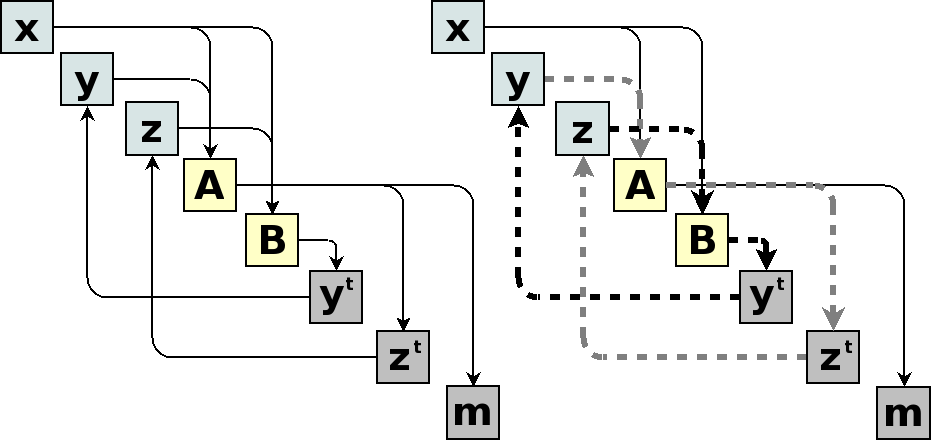
\includegraphics[width=.75\textwidth]{images/dsm_simple}
        \caption{Graph and matrix based DSM specifications for a notional analysis \label{fig:dsm_simple}}
        \end{center}
    \end{figure}

    Since a DSM describes a square adjacency matrix, it can be represented in an equivalent directed graph where nodes represent analysis tools and 
    edges represent information exchange between those tools. An alternate matrix based syntax, called a 
    Functional Dependence Table (FDT), was proposed by Michelena and Papalambros. 
    FDT represents the relationship between functions, including objectives and constraints, and their values\cite{Michelena1997}. Similar to DSM
    FDT also describes an adjacency matrix of a graph. Unlike the DSM graph, however, a FDT graph is an undirected 
    graph where nodes can represent analysis tools, objectives, or constraints. Edges between nodes represent a dependence on the same 
    variable value. By searching the FDT graph for clusters of totally connected nodes Wagner and Papalambros were identify groups of 
    analysis tools that were all dependent on the same input variables and used that to make partitioning decisions \cite{Wagner1993}. FDT retains 
    a greater portion of the information in the problem formulation, but it is still not complete. It ignores information about feedback coupling 
    between codes. 

    It is possible to combine the syntax of an FDT and a DSM by making a small extension to a traditional DSM specification. Normally, a DSM is given 
    with analysis tools as nodes and variable dependencies given as edges. Lamb and Martins included the variables, objectives, and constraint functions
    as nodes in an Extended DSM (XDSM)\cite{Lambe2012} in order to capture a more complete problem formulation for MDAO problems. With XDSM 
    it is possible to specify a complete problem formulation. Lu and Martins developed a process to perform ordering and partitioning on the fundamental 
    problem formulation specified by XDSM in order to achieve significant reductions in computational costs for large scale optimization problems. 
    Figure \ref{fig:dsm_full} illustrates the same notional analysis as in Figure \ref{fig:dsm_simple} represented as an XDSM.

    \begin{figure}[!hbp]
        \begin{center}
        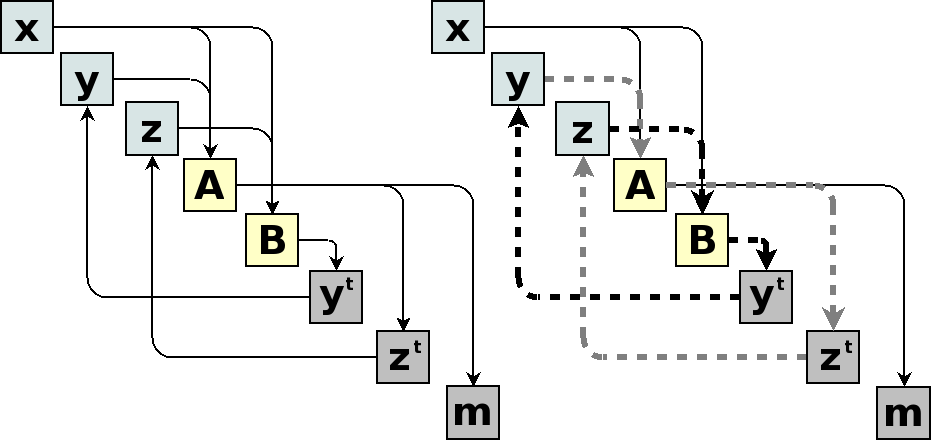
\includegraphics[width=.75\textwidth]{images/dsm_simple}
        \caption{[TODO: Generate XDSM]Extended DSM graph for a notional analysis \label{fig:dsm_full}}
        \end{center}
    \end{figure}